%\documentclass[12pt]{article}
\input{/Users/joshyv/Research/misc/latex_paper.tex}
\newcommand{\f}{f_{\thet}}
\newcommand{\g}{g_{\thet}}
\newcommand{\x}{\ve{x}}
\newcommand{\y}{\ve{y}}
\newcommand{\h}{\ve{h}}
\newcommand{\xT}{\x} %whole time series
\newcommand{\yT}{\y}
\newcommand{\fhat}{\widetilde{f}_{\thet} \big(\x_t^{(l)} | \x_{t-1}^{(m)}\big)}
\newcommand{\ppi}{\pi_{\thet}}
\newcommand{\phat}{\widehat{P}_{\thetn}(F_v | \Ca_t)}
%\usepackage[hypertex]{hyperref}    %for LaTeX
\usepackage{hyperref}               %for pdfLaTeX

\title{Inferring connectivity from imaging activity}
\author{Joshua Vogelstein, some others,  Liam Paninski}

\begin{document}

\maketitle

\begin{abstract}
We present Bayesian framework for inferring connectivity in a network
of coupled neurons, observed simultaneously using calcium imaging.

\end{abstract}

\section{Introduction}
Our goal is to estimate the connection matrix of a population of neurons from simultaneously imaging their activity. 


\section{Model}
\subsection{Single neuron model}

We assume that we have a discrete time model, with time step size $\Delta$ and $T$ total time steps. In each time step, the neuron can emit any non-negative number of spikes, i.e., $n_t \in \{0,1,2,\cdots\}=\mathbb{N}_0$.  The spiking is governed by a Poisson process with rate $\lambda_t \Delta$, where $\lambda_t$ is given by: 

\begin{align} \label{eq:1neur}
\lambda_t &= \exp\{b + \ve{k}' \ve{s}_t + \omega h_t\} \\
h_t - h_{t-1}&= - \frac{\Delta}{\tau_h} h_t + n_{t-1} + \sigma_h \sqrt{\Delta} \varepsilon
\end{align} 

%\noindent where $b$ sets the baseline firing rate, $\ve{k}$ is a linear filter operating on the external stimulus, $\ve{s}_t$, $\omega$ is the weight on the spike history term, $h_t$. The spike history term jumps instantaneously after a spike, and then decays with time constant $\tau_h$ back to zero. Spiking induces a change in the intracellular calcium concentration, $\Ca$, which is measured using fluorescence, $F_t$: 

calcium model:

\begin{align}
\Ca_t - \Ca_{t-1} &= -\frac{\Delta}{\tau_c}(\Ca_t + \Ca_b) + A n_t + \sigma_c \sqrt{\Delta} \varepsilon, 
\end{align}

observation model:
\begin{align} \label{eq:1obs}
F_t = \alpha S(\Ca_t) + \beta + (S(\Ca_t)+\sigma_F) \varepsilon_t
\end{align} 

\noindent where $S(x)=x^n/(x^n+k_d)$ is the standard Hill equation,  the $\varepsilon$'s indicate standard normal random variables.


\subsection{Multiple neuron model} \label{sec:popmod}

We assume the firing rate for neuron $i$, $\lambda_{i,t} \Delta$, is given by:

\begin{align} \label{eq:poisson}
\lambda_{i,t} &= f(b_i + \ve{k}_i'\ve{s}_t + \sum_{j=1}^N \omega_{ij} h_{j,t}) \\
h_{i,t}-h_{i,t-1} &= -\frac{\Delta}{\tau_{h_i}} h_{i,t} + n_{i,t-1}  + \sigma_{h_i} \sqrt{\Delta} \varepsilon,
\end{align} 

\noindent where each $h_{i}$ corresponds to the spike history term associated with neuron $i$, and has an associated time-constant, $\tau_i$.  The input each neuron recieves, therefore, is the sum of spike history terms from all neurons (including itself).  Thus, $\ve{\omega}$ = $\{\omega_{ij}\}$ = $\{\omega_{11}$, $\omega_{12}$, \ldots, $\omega_{1N}$, $\ldots$, $\omega_{NN}\}$ comprises the weight matrix for these neurons.

calcium model:

\begin{align}
\Ca_{i,t} - \Ca_{i,t-1}&= -\frac{\Delta}{\tau_{c_i}} (\Ca_{i,t} + \Ca_{b_i}) + A_i n_{i,t} + \sigma_{c_i} \sqrt{\Delta} \varepsilon, 
\end{align}

observation model:
\begin{align} \label{eq:2obs}
F_{i,t} &= \alpha_i S(\Ca_{i,t}) + \beta_i + (S(\Ca_{i,t}) + \sigma_{F_i}) \varepsilon,
\end{align} 

Note that we assume that $S(\cdot)$ is the same for each neuron (i.e., the nonlinear function is the same for each neuron, because the parameters are a function of the indicator, not the neuron).  Further note that we assume (for now) that the noise on the calcium and observation for each neuron is independent (an assumption that we will probably want to relax later).


\section{Mathematical Background}
To estimate $\ve{\omega}$, we adopt a state-space framework.  More specifically, let $y_t$ be the observations, and $x_t$ be the \emph{hidden states}.   We then have:

\begin{align}
\y_t &\sim \g (\y_t | \x_t) \label{eq:y_t} \\
\x_t &\sim \f (\x_t | \x_{t-1}) \label{eq:x_t}
\end{align}

\noindent where $\g(\cdot)$ and $\f(\cdot)$ indicate the \emph{observation} and \emph{transition} distributions, respectively (and we have adopted the shorthand notation $\f(\cdot)=f(\cdot | \thet)$.  Letting $\ve{X}_t$ = $\{X_{i,t}\}$ = $\{X_{1,t}, \ldots, X_{N,t}\}$, for the above model, we have $\y_t=\ve{F}_t$, $\x_t=\{\ve{n}_t, \ve{h}_t, [\textbf{Ca}^{2+}]_t\}$, and $\thet=\{\ve{\alpha}$, $\ve{\beta}$, $\ve{\tau_c}$, $\ve{\Ca_b}$, $\ve{\sigma_c}$, $\ve{b}$, $\{\ve{k}_i\}$, $\ve{\omega}$, $\ve{\tau_h}, \ve{\sigma}_h\}$.   Note that given the above model, $\y_t \in \Re_+^N$, i.e., each $y_t$ is a non-negative real number, and $\x_t \in \Re_+^{2N} \times \{0,1\}^N$, i.e., $\x_t$ lies in a $3N$-dimensional space, where $2N$ dimensions are non-negative real numbers ($\Ca_t$ and $h_t$ for each neuron), and the rest are binary ($n_t \in \{0,1\}$ for each neuron).  Thus, we have a ``hybrid'' system, in that some of our hidden states are continuous, and others are discrete.  We may now formally state our goal as:

\begin{align} \label{eq:max}
\widehat{\thet} = \argmax_{\thet} \p(\yT) = \argmax_{\thet} \int \p(\yT, \xT) d\xT 
\end{align}

\noindent where, we have introduced the notation, $\yT=\y_{0:T}$, and $\p(\yT, \xT)$ may be factored as: 

\begin{align}
\p(\yT, \xT) = \ppi (\x_0) \prod_{t=1}^T \g(\y_t | \x_t) \f(\x_t | \x_{t-1}) 
\end{align}

\noindent where $\ppi(\x_0)$ is the initial distribution of $\x$.  Sadly, for our model, integral in \eqref{eq:max} is computationally intractable. Therefore, we adopt an EM approach:

\begin{align}
\widehat{\thetn} &= \argmax_{\thetn} \Q\\
\Q &= E_{p_{\theto}(\xT | \yT)} \ln p_{\thetn} (\yT, \xT)% \nonumber \\ &
= \int p_{\theto} (\xT | \yT) \ln p_{\thetn} (\yT, \xT) d\xT 
\end{align}

Because we have a state-space model, the above integral may be simplified:

\begin{multline} \label{eq:Q2}
\Q = \int p_{\theto}(\x_0 | \yT)  \times \ln \pi_{\thetn}(\x_0) d\x_0 + \\
\sum_{t=1}^T \iint p_{\theto} (\x_t, \x_{t-1} | \yT) \times \ln f_{\thetn}(\x_t | \x_{t-1}) d\x_t d\x_{t-1} + \\
\sum_{t=0}^T \int p_{\theto} (\x_t | \yT) \times \ln g_{\thetn}(\y_t | \x_t) d\x_t
\end{multline}

As we have a nonlinear observation model, and nonlinear transition model, the integrals in \eqref{eq:Q2} are intractable as well, so they must be approximated. We adopt a monte carlo strategy, in which we approximate the above integrals with sums. This requires approximating the continuous valued hidden states with discrete valued hidden states. The key is to be able to estimate the pairwise joint conditionals:

\begin{align}
p_{\thet} (\x_t, \x_{t-1} | \yT) \approx \sum_{k,m=1}^k \widetilde{p}_{\thet} \big(\x_t^{(k)}, \x_{t-1}^{(m)} | \yT\big) \delta_{\x_t^{(k)}}(\x_t) \delta_{\x_{t-1}^{(m)}} (\x_{t-1})
\end{align}

\noindent where $\delta_{\x}(\cdot)$ denotes the Dirac mass at point $\x$, and $\widetilde{p}_{\thet}(\x_t^{(k)},  \x_{t-1}^{(m)} | \yT)$ is computed pointwise for each $\x_t^{(k)}$ and $\x_{t-1}^{(m)}$, and then normalized such that $\sum_{k,m=1}^k \widetilde{p}_{\thet}(\x_t^{(l)} | \x_{t-1}^{(m)})=1$. From this approximation, we can also estimate the marginal conditionals and initial distribution, by integrating out $\x_{t-1}$. The key is to efficiency discretize the space, so $L$ is small and the approximation is still good.  We adopt a Monte Carlo strategy, in which we represent the pairwise joint conditionals as a product of terms:

\begin{align}
 \phat \big(\x_t^{(l)}, \x_{t-1}^{(m)} | \yT\big) = \phat \big(\x_t^{(l)} | \yT\big) \frac{\fhat w_{t-1}^{(m)}} {\sum_{m=1}^L  \fhat w_{t-1}^{(m)}}
\end{align}

\noindent where $w_t^{(l)}$ is defined by

\begin{align}
\p(\x_{t} | \y_{1:t}) = \sum_{l=1}^L w_t^{(l)} \delta_{\x_{0:t}^{(l)}} (\x_{0:t})
\end{align}

The maximize efficiency, therefore, we aim to choose $\x_t^{(l)}$'s to make their associated weights, $w_t^{(l)}$'s approximately equal. In the next section, we describe a number of algorithms, with increasing complexity and (hopefully) utility. 

Thus, it should be clear from the above that ideally, one would ideally like to sample jointly from $p(\x_t | \x_{t-1}, \y_t)$.  As this is so high dimensional (more specifically, $3N$ dimensions), the importance sampling idea breaks down (as it is incapable of approximating a high dimensional space with a small number of particles).  Therefore, we develop a number of approaches to combat this curse of dimensionality.

%We utilize a Sequential Importance Resampling (SIR) strategy in which we choose as the importnace function the one-step-ahead sampler and perform stratified resampling as needed.  

%\subsection{single-neuron dynamics}
%
%Thus, we have a transition and observation distirbutions:
%
%\begin{align}
%p(\x_t | \x_{t-1}) &= p(\Ca_t | \Ca_{t-1}, n_t) p(n_t | h_t) p(h_t | h_{t-1}, n_{t-1})\\
%p(\y_t | \x_t) &= p(F_t | \Ca_t),
%\end{align}
%
%\noindent where the above distributions are defined as:
%
%\begin{align}
%p(\Ca_t | \Ca_{t-1}, n_t) &= \mathcal{N}(\Ca_t; a_c \Ca_{t-1} + b + A n_t; \sigma_c^2 \Delta) \\
%p(n_t | h_t) &= \mathcal{B}(n_t; \lambda_t) \\
%p(h_t | h_{t-1}, n_{t-1}) &= \mathcal{N}(h_t; a_h h_{t-1} + n_{t-1}, \sigma_h^2 \Delta)\\
%p(F_t | \Ca_t) &= \mathcal{N}(F_t; \alpha S(\Ca_t) + \beta, (S(\Ca_t) + \sigma_F)^2)
%\end{align}

\subsection{population dynamics}

plugging model described in section \ref{sec:popmod} into \eqref{eq:y_t} and \eqref{eq:x_t}, we have:

\begin{align}
p(\x_t | \x_{t-1}) &= \prod_{i=1}^N p(\Ca_{i,t} | \Ca_{i,t-1}, n_{i,t}) p(n_{i,t} | \h_t) p(h_{i,t} | h_{i,t-1}, n_{i,t-1})\\
p(\y_t | \x_t) &= \prod_{i=1}^N p(F_{i,t} | \Ca_{i,t})
\end{align}

\noindent where $\h_t=h_{1,t}, \ldots, h_{N,t}$ and the above distributions are defined by

\begin{align}
p(\Ca_{i,t} | \Ca_{i,t-1}, n_t) &= \mathcal{N}(\Ca_{i,t}; a_{c_i} \Ca_{i,t-1} + b_i + A_i n_{i,t}; \sigma_{c_i}^2 \Delta) \\
p(n_{i,t} | \h_{i,t}) &= \mathcal{B}(n_{i,t}; \lambda_{i,t}) \\
p(h_{i,t} | h_{i,t-1}, n_{i,t-1}) &= \mathcal{N}(h_{i,t}; a_{h_i} h_{i,t-1} + n_{i,t-1}, \sigma_{h_i}^2 \Delta)\\
p(F_{i,t} | \Ca_{i,t}) &= \mathcal{N}(F_{i,t}; \alpha_i S(\Ca_{i,t}) + \beta_i, (S(\Ca_{i,t}) + \sigma_{F_i})^2)
\end{align}

\noindent and we have introduced $a_{c_i}=1-\Delta/\tau_{c_i}$, $b_i=-\Delta \Ca_{b_i} / \tau_{c_i}$, and $a_{h_i}=1- \Delta / \tau_{h_i}$, for brevity.


\section{Results}

\subsection{Main Result}
Our goal is to infer the probability of each neuron spiking at any time, conditioned on \emph{all} the fluorescence measurements from the entire population of neurons: $\p(\bn_t | \bF_{1:T})$ for $t = 1. \ldots, T$.  As the uncertainty is non-Gaussian (due to the assumed Bernoulli distribution governing spikes), and the dynamics are nonlinear (due to the saturation of fluorescence, $S(\cdot)$, standard linear-Gaussian filtering is inadequate for this model.  Instead, we generalize our previous result \cite{BJ08}, in which we utilized sequential Monte Carlo methods to develop a model-based optimal nonlinear filter.  Very briefly, in that work, we used a particle filter to recursively infer $\p(n_t | F_{1:t})$, for $t=1, \ldots, T$, and used a particle smoother to recurse backwards, obtaining $\p(n_t | F_{1:T})$ \cite{DoucetGordon01}.  By embedding this particle-filter-smoother (PFS) into an expectation-maximization framework, we can iterate inferring the hidden spike trains and learning the parameters \cite{DoucetGordon01}.  Importantly, in that work, we modeled each neuron as an independent generalized linear model (GLM).  In contrast, here we model the neurons as coupled GLMs \cite{Paninski04c, TruccoloBrown05, Pillow08}.  Thus, we can condition the probability of each neuron spiking at any time on the spike history of all observed neurons. More precisely, we proceed as described in Algorithm \ref{alg:1}.  Note, we have assumed that all the parameters governing $\bF$ and $\bC$ have been estimated already, using the GLM PFS described in \cite{BJ08}.

\begin{algorithm}
\caption{Pseudocode for inference and learning for a population of simultaneously observed neurons.  } \label{alg:1}
\begin{algorithmic}[1]
\WHILE[$j$ indexes iterations]{$j=1, \ldots$} 
\FOR[$i$ indexes neurons]{$i=1$ to $m$}
\STATE Let $\tbx_{i,t}^{(j)}=\big[\bx_t,\: \tbh_{\backslash i,t}^{(j)}\big]'$, where $\tbh_{\backslash i, t}^{(j)}=E[\bh_{\backslash i,t}^{(j)} | \bF_{1:T}]$ and $\bh_{\backslash i,t}=\{h_{1,t}, \ldots, h_{i-1,t}, h_{i+1,t}, \ldots, h_{m,t}\}$
\STATE Let $\tbk_i^{(j)}=\big[\bk_i^{(j)},\: \ve{\omega}_{\backslash \bi}^{(j)}\big]'$, where $\ve{\omega}_{\backslash \bi}=\{\omega_{i,1}, \ldots, \omega_{i,i-1}, \omega_{i,i+1}, \ldots, \omega_{i,m}\}$
\STATE Infer $P_{\bth^{(j)}} (\{C,n,h\}_{i,t}^{(j+1)} | \bF_{1:T}) \: \forall t$ where $n_{i,t} \sim $ Ber$\big(n_{i,t}; \big(\tbk_i^{(j)}\big)' \tbx_{i,t}^{(j)}\big)$ using GLM PFS as described in \cite{BJ08}
\ENDFOR

\FOR{$i=1$ to $m$}
\STATE  Estimate $\tbk_i^{(j+1)}=\big[\bk_i^{(j+1)}, \: \ve{\omega}_{\backslash \bi}^{(j+1)}\big]$ using GLM PFS as described in \cite{BJ08}
\ENDFOR

\ENDWHILE
\end{algorithmic} 
\end{algorithm}

\begin{figure}[h!] 
\begin{center} 
%\epsfxsize=4.4in 
%\epsfysize=2.4in \epsffile{SimConnector.eps} 
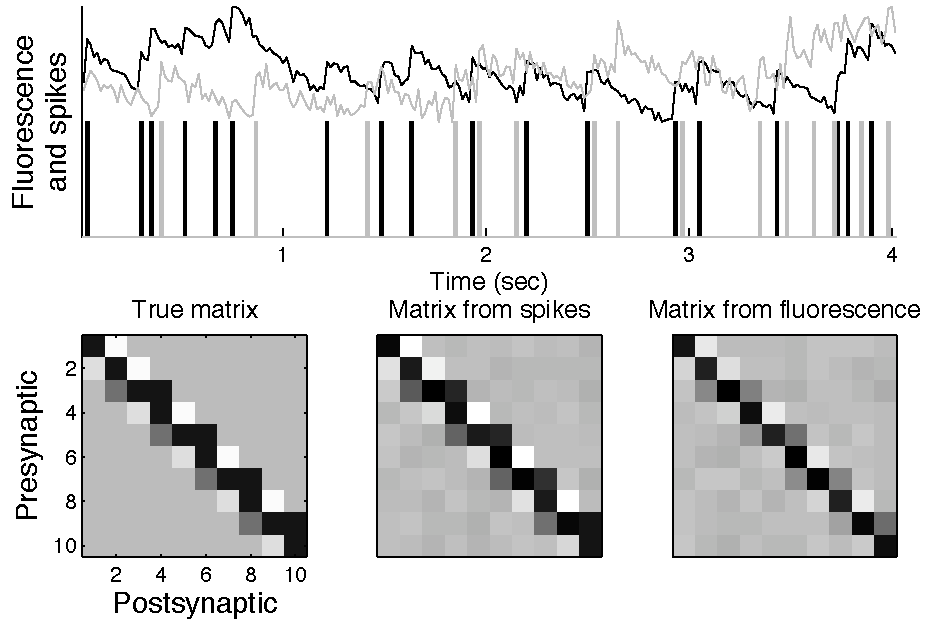
\includegraphics[width=0.7\linewidth]{../figs/SimConnector} 
\caption{Inferring network connectivity given noisy simulated calcium fluorescence data. Our main result is that we can infer network connectivity given only short sequences of observations ($<10$ min), for small populations of neurons ($\sim 10$), given reasonable assumptions on spike rate ($\sim 5$ Hz), observation frequency ($60$ fps), and observation noise. \textbf{Top}: True spikes and observed noisy calcium fluorescence traces for two cells in the simulated network.  Calcium data sampled at 60 Hz.  (Only four seconds of a longer experiment are shown here, for clarity.)  \textbf{Bottom}: True connectivity matrix; connectivity matrix estimated given the fully observed spikes; and connectivity matrix estimated given just the noisy calcium data, given about 2000 spikes/neuron.  White denotes excitatory connections; black denotes inhibition; the same grayscale map is used for each panel.  A small simulated network was used for illustration purposes.  Each cell inhibited itself following each spike (a relative refractory effect) and excited or inhibited its nearest neighbors; the strength and time constant of these excitatory terms were chosen to mimic the experimentally determined parameters (a spike in one cell modulates the instantaneous firing rate in another cell by no more than $5\%$ -- $10\%$).  No external drive was applied to the network; i.e., only spontaneous network dynamics are observed here.  Note that it is somewhat harder to estimate the connectivity map given noisy calcium data than the true spike trains (specifically, some of the inhibitory connections are slightly underestimated in the right panel); nonetheless the correct connectivity is obtained with only a few minutes of calcium data.} \label{fig:gibbs} 
\end{center}
\end{figure}


\subsection{Embedded MCMC improves inference}
To test the performance for inference of neural connectivity in a neural population, we simulated such inference in conditions close to such expected in real data.
Specifically, we solve connectivity inference for a network of simulated spiking neurons, constructed closely following empirical data known about the real neural networks in the cortex. We assume a population of neurons that are spontaneously firing action potentials.
While it is known, that the functional connectivity weights in general do not properly reflect anatomical connectivity in a circuit, we will show that for the above system of spontaneously firing neurons the direct correspondence, indeed, exists, and anatomical connectivity is properly recovered via functional connectivity weights.

Functional connectivity may fail to faithfully represent anatomical circuit structure if false correlations are present between different neurons, induced e.g. by common inputs, or if the dynamics of neural population is entirely concentrated on a low-dimensional subspace of the full configurational space $H$. Note that these two statements are, in a sense, different ways of stating the same condition: if activity of different neurons is tightly correlated, their dynamics is concentrated on a low-dimensional plane; and vice-versa - concentration of dynamics onto a low-dimensional plane will be perceived as correlation in activity of different neurons. (In turn, low dimensionality of the neural dynamics may be caused by different factors, including common input, small subset of command neurons driving the circuit, or even emergent property of a network.) Low dimensionality of the neural dynamics results in that the inference problem Eq.(\ref{eqn:loglik:definition}) becomes underdetermined, i.e. there may exist directions in $W$ along which connectivity is not constrained by activity data (i.e. directions orthogonal to the subspace of all observed neural activity configurations), or is poorly constrained. This, naturally, leads to $W$ being poorly defined along these directions. The necessary condition for good correspondence between functional connectivity weights $W$ and anatomical connectivity, therefore, is {\em full-dimensionality} of the observed neural dynamics. In case of spontaneously firing system of neurons this condition is, in fact, satisfied by many independent neuron-ignitions, thus, fully sampling possible directions in the configurational space $H$. If spontaneously active preparation by itself fails to display sufficient degree of independence between randomly firing neurons (e.g. if low-dimensionality of the activity subspace is the emergent property of studied circuit), such pattern may be induced by randomly activating subsets of neurons via ChR2 [...] or glutamate uncaging.

We also note that the correlations induced by secondary and so on synaptic transmissions (such as when neuron $A$ results in firing of neuron $B$, which in turn results in firing by neuron $C$), are all properly resolved in GLM-fitting process via the so called explaining-away process. In other words, because we do not just identify correlations between neural firings with the functional connectivity weights $w^{kk'}$, but instead statistically fit a model of neural interactions, if found weights between neurons $A$ and $B$, and $B$ and $C$ are sufficient to explain the correlation between $A$ and $C$, the weight connecting $A$ and $C$ will not appear in the model - the correlation between $A$ and $C$ was ``explained away'' by correlations between $A$ and $B$, and $B$ and $C$. By this, the multi-synaptic firing patterns do not confuse our estimation process.

We prepared a small network of $N=50$  neurons randomly sparsely connected, and firing stochastically with the base firing rate of about 5Hz. Each neuron was modeled with GLM as a linear-nonlinear driven Poisson spike generator, as described above
\begin{equation}\label{eqn:glm-def}
\begin{array}{l}
P(n^k_{t+1}|\{h_{t+1}\})=$Poiss$(\lambda^k_{t+1}\Delta t) \\
\lambda^k_{t+1}=g(J^k_t)=g(b_0+\sum_{\tau>0}w^{k,k'}_{\tau}n^{k'}_{t-\tau}),
\end{array}
\end{equation}
with exponential transfer function $g(J)=\exp(J)$. We assumed no external modulating input $X_{ext}(t)$.

The network was divided into excitatory and inhibitory components.
Neurons in such components were either entirely excitatory or inhibitory; i.e., all connections outgoing from such neuron were either all simultaneously positive (excitatory) or negative (inhibitory). Excitatory neurons were randomly connected with each other and the inhibitory neurons with probability $f_c=0.1$ (observed probability for a local connection between nearby neurons in the cortex [**]). The synaptic weight of each connection $v$, as defined by max EPSP amplitude, were generated from exponential distribution with mean $0.5 \mu V$ [**] (we neglected here the ``heavy tail'' of the distribution of synaptic weights observed in some datasets [**]).
While synaptic weights are typically measured in PSP units of $\mu V$,
in GLM model connections are measured in log-rate units of Eq.(\ref{eqn:glm-def}).
In other words, GLM weights describe the {\em change in probability of neuron $k$
to fire given neuron $k'$ has firing before}.
By utilizing this definition, we may convert a PSP weight $v_{EPSP}$ for a neuron $V_{base}$ below spike-triggering threshold into the GLM weight as $v_{GLM}\approx v_{EPSP}/V_{base}$. In other words, $V_{base}/v_{EPSP}$ spikes are required to push neuron over the threshold. Given the definition of the firing rate in (\ref{eqn:glm-def}), this
leads to the following equation for the log-rate couplings $w^{kk'}$
\begin{equation}\label{eqn:convert}
w^{kk'}=\ln(-\ln(\exp(-f^k \Delta t)-v^{kk'}_{EPSP}/V_{base})/\Delta t/f^k),
\end{equation}
where $f^k$ is the base ``stochastic'' firing rate of neuron $k$.

20\% of all neurons were taken to be inhibitory [**]. Interneurons were randomly connected among themselves and to excitatory neurons with the same frequency $f_c=0.1$ as above. The strength of the inhibitory connection was drawn from the exponential distribution with mean chosen to balance excitatory and inhibitory currents, and to achieve the final firing rate close to the base firing rate $f=g(b_0)$. Connection strengths were thus converted to log-rate units using Eq.(\ref{eqn:convert}), where $w^{kk'}$ was finally multiplied by -1 to reflect inhibition.

To generate a sequence of spikes in this population, we simulated activity of the network forward in time computing currents injected into each cell from all previous spikes of all neurons. Each spike was assumed to inject the same PSP waveform, described by a temporal filter $h_{PSP}$ [DIAGRAM] modeled as the difference of two exponentials with the rise time of $1ms$ and decay time of $10ms$ [**]
\begin{equation}
J^k_{t, inject} = \sum_{k'\neq k}w^{kk'}\sum_{\tau>0}
h_{PSP}(\tau) n^{k'}_{t-\tau}.
\end{equation}
(Given $1ms$ time step of our simulation, and the fact that
a signal in a local cortical circuit of the size of $\sim 1mm$
would suffer $\leq 1ms$ time lag, we neglect delays
in this simulation.) Additionally, each neuron exhibited refractory current with waveform $h_{REFR}$ [DIAGRAM] modeled with exponential with decay time of $5ms$ [**]
\begin{equation}
J^k_{t,{refr}} = \Omega^k \sum_{\tau>0}h_{REFR}(\tau) n^{k}_{t-\tau}.
\end{equation}
The network was then thus simulated forward in time with step of $\Delta t=1ms$. All neurons were assumed to be electro-physiologically similar (i.e. have the same PSP profiles, $\Omega$ and base firing rate, etc.) Spikes were generated at each time according to Bernoulli distribution
$n^k_t=$Bernoulli$[g(J^k_{t,spont}+J^k_{t,refr}+J^k_{t,inject})\Delta t]$.

Given a sequence of spikes, the fluorescence observations were generated using the setup in [VogPan]. Parameters for the model were chosen in accordance to our experience of analyzing a few actual cells [**]. Specifically, calcium decay time constant was $\approx 0.25 s$, the ratio of per-spike calcium influx to stochastic fluctuations in calcium concentration was $\approx3:1$,
and the background of calcium concentration was chosen to be about 30\% of per-spike calcium influx, thus corresponding to typical relatively low SNR of 1:3. Photon count per measurement was taken to be $\approx 3\cdot 10^4$. The population of cells was generated with these parameters while assuming that all parameters may vary by at least 30\% from cell to cell. Thus, we generated fluorescence for each cell using its unique cell of parameters, and produced sampled observations at frame-rate of 33Hz or 66Hz. [PARAMS-TABLE]

\subsection{Including a sparse prior}
%\input{prior}

\subsection{Data}

\section{Other algorithms}
XXX: this section is still under much development


\subsection{Default algorithm: see \cite{BJ08} for details} \label{sec:default}

\begin{description}
\item[Initialization]: \\
\begin{enumerate}
\item Manually define an ROI around each neuron.
\item Average pixel intensity from all pixels in a frame to obtain $F_{i,t}$, i.e., the fluorescence intensity indexed by cell indentity $i$ and frame number $t$.
\item Separately for each neuron, implement PFS as described in \cite{BJ08} (ie, with all cross-coupling terms turned off). 
\end{enumerate}
\item[Recursion]: \\
\begin{enumerate}
\item For each neuron, let the input, $\bu_{i,t} = [\bs_t, \{\widetilde{\h}_{i,t}\}]$, where $\{\widetilde{\h}_{i,t}\}= \{E[\h_{i,t} | \bF]$ for all $i\}$.
\item Use PFS from \cite{BJ08} to learn $\ve{\omega}$ 
\end{enumerate}
\end{description}

\subsection{Population PF} \label{sec:PopPF}

\begin{enumerate}
\item same as \ref{sec:default}
\item same as \ref{sec:default}
\item particle filter step: this generalizes \ref{sec:default} by sampling not just on self-histories, but also cross-histories.  because the transition distribution factorizes as above, we can sample from the optimal one observation ahead sampler, ie, $p(\x_t | \x_{t-1}, \y_t)$ (by approximating the likelihood term as a Gaussian in $\Ca_{i,t}$). in particular, to sample spikes after integrating out everything, one is left with:

\begin{align}
n_{i,t} \sim p(n_{i,t} | \h_t) \mathcal{N}(\Ca_{i,t}; \mu_{c_{i,t}}, \sigma_{c_{i,t}}^2)
\end{align}  

\noindent where $\mathcal{N}(\Ca_{i,t}; \mu_{c_{i,t}}, \sigma_{c_{i,t}}^2$ is a Gaussian approximation to the product of the likelihood and calcium update terms.  

\item same as \ref{sec:default}
\item estimate parameters using standard EM stuff as in \cite{BJ08}
\end{enumerate}

it's not obvious whether this approach will outperform the approach outlined in \ref{sec:default}

\subsection{Gibbsish Population PF} \label{sec:G1PF}

this generalizes \ref{sec:PopPF}, by sampling conditioned not just on spike histories, but also on spike futures from other neurons.  in particular, we want to sample spikes for one neuron conditioned on its own past spikes, and \emph{all} spikes from all other neurons.  having already completely an iteration, we now sample spikes according to:
\begin{align}
n_{i,t} \sim p(n_{i,t} | \h_t, \h_{\backslash i, t+1}) \mathcal{N}(\Ca_{i,t}; \mu_{c_{i,t}}, \sigma^2_{c_{i,t}})
\end{align}

\noindent where $\h_{\backslash i,t+1}=\{h_{1,t+1}, \ldots, h_{i-1,t+1}, h_{i+1,t+1}, \ldots, h_{N,t+1}\}$.  we compute this using the method described in \cite{PillowLatham07}.  For future spikes, we let the posterior mean of the spike train from the previous EM iteration correspond to future spikes.

\subsection{Gibbser Population PF} \label{sec:G2PF}

this generalizes \ref{sec:G1PF}, by sampling not just sampling based on previous EM iteration's mean posterior spike train, but actually doing a proper gibbs step within each forward pass. in particular, we do the sampling as described in \ref{sec:G1PF} to initialize, and obtain a spike train for each neuron.  we then iterate, sampling for each neuron, conditioned on the entire spike trains for other neurons.  by gibbs, we will eventually converge to having sampled jointly from them all. i am not convinced that this is a particularly useful generalization of the \ref{sec:G1PF}.


\subsection{Metropolis-Gibbs Population PF} \label{sec:G3PF}

this generalizes \ref{sec:G2PF}, by placing the Gibbs sampler just described into a MCMC approach.  more specifically, we proceed as follows. for each neuron:

\begin{enumerate}
\item generate $M-1$ particles, sampling according to $p( n_{i,t} | \h_t, \h_{\backslash i, t+1}, F_{i,t})$ as described in \ref{sec:G2PF}.  
\item add current path to population of particles and compute appropriately normalized transition probabilities
\item use standard forward-backward sampling algorithm for HMM's to sample $\x^{\ast}$ from this augmented space
\item compute $q(\x^{\ast})$, the probability of sampling $z$ using a forward-backward recursion
\item compute probability of acceptance, $r= \frac{q(\x) p(\x^{\ast})}{q(\x^{\ast})p(\x)}$, where $\x$ is the current path and $p(\x^{\ast})$ is the posterior
\end{enumerate}

we iterate this step until we accept a new spike train for a particular neuron, and then repeat for all subsequent neurons. alternately, we could randomly choose a neuron after each iteration.  i have no idea which approach would be better.

\paragraph{speeding things up}

as this probably will take a while, we can do a number of things to speed it up

\begin{itemize}
\item skip generating particles step sometimes, ie, keep sampling from a particular HMM until prob of acceptance gets too small
\item do an increment/decrement thing.  in other words, after generating the first set of particles, with each additional acceptance, we simply eliminate a path (based on its likelihood).  thus, we must only generate $M-1$ extra particles once.
\item instead of using the standard hmm sampling to generate a new proposal, use Viterbi for PF (as described in \cite{GodsillWest01}, or the fast version of that approach (as described in \cite{KlaasFreitas05} to generate a possible new sequence. then, if that one is not accepted, use standard hmm sampling to generate other proposals.
\end{itemize}

\subsection{Ways we might make stuff better}

these ideas potentially improve on all the above ideas.

\begin{enumerate}
\item Improved observation model --- Identify ROI for each neuron using some ImageJ plug-in (or other such method).  Instead of equally weighting all pixels, initialize pixel weights with first eigenvector computed using SVD, and then proceed as before.  upon constructing SS, update spatial filter weights along with other parameters.  An analysis of the kind of spatial filters should facilitate parameterizing the filter (potentially as a mixture of Gaussians).  Alternately, an appropriate regularizing kernel may help. Note that if two or more neurons are in the same ROI, the observation model must be modified somewhat (but I'm not putting those details in here at this time) 
\item Improved transition model --- The most obvious improvement would be to allow additional time constants for the dynamics (either calcium or fluorescence).  Perhaps the best way to decide what to include would be to take data for which we have both images and ephys, and fit a couple parametric models, and do cross-validation to compare which is best.  The options would include: (i) an additional calcium state, (ii) temporal dynamics for the fluorescence, (iii) no noise on calcium, or (iv) some combination of the above.  
\item Rao-blackwellized Particle Filter (RBPF) --- This would amount to having a mixture of kalman filters (MKF), each conditioned on a particular spike train.  As far as reducing unnecessary variance, I think it would be hard to justify not incorporating this into our model (see \cite{Chen00} for details). Note, however, that in the limit as $N \rightarrow \infty$, the particle approximation is perfect, whereas the RBPF (or MKF) is not, because we must estimate the likelihood as a Gaussian function of $\Ca$.  
\end{enumerate}

\subsection{these are not very good ideas, but i thought they were potentially worth writing down}

\begin{enumerate}
\item Improved resampling --- we could use a number of tricks here
\begin{itemize}
\item  sample $N_p' > N_p$ particles, but only resample using $N_p$ particles, aka, prior boosting (see \cite{Green95,CarpenterFearnhead99} for details).
\item  Rejection sampling --- We do not resample, but rather, only accept particles at each time. See \cite{Chen03} Section E for a summary  (and refernces therein for details). 
%first, we sample $\x_{t-1}^{(i)}$ with probability $\gamma_t^{(i)}$, where
%\begin{align}
%\gamma_t^{(i)} &= \frac{C_t^{(i)}}{N_p C_n}
%C_n &\approx \frac{1}{N_p^2} \sum_{i,j=1}^{N_p} p(\y_t | x_{t|t-1}^{(ij)})
%C_n^{(i)} \approx \frac{1}{N_p} \sum_{j=1}^{N_p} p(\y_t | \x_{t|t-1}^{(ij)})
%\end{align}
%
%\noindent and then generate a new sample, $\z_t$, from $q(\cdot)$, which is accepted only if $u\leq \alpha(\z_t)$, where 
%\begin{align}
%\alpha(\z_t) = \frac{p(\y_t | \z_t) p(\z_t | \x_{t-1}^{(i)}) / q(\z)} {\sup_{\z} \{p(\y_t | \z_t) p(\z_t | \x_{t-1}^{(i)}) / q(\z)\}}
%\end{align}
%\noindent where $\z_t$ is the newly sampled particle, $q(\cdot)$ is the proposal distribution, and $u \sim \mathcal{U}(0,1)$
\item  robust weighting (to handle outliers) (see review on particle filters)
\end{itemize}  

\item MCMC with particle filtering --- there are a number of ways to do this kind of thing
\begin{itemize}
\item RESAMPLE-MOVE --- 
\item Metropolized Gibbs sampler --- see \cite{Liu96} for details
\end{itemize} 

\item data-augmentation for parameter estimation (ie, iterate estimating $p(\x | \y, \thet)$ and $p(\thet | \y, \x)$ to eventually converge to $p(\x, \thet, \y)$).
\item use algorithm in continuous-time particle-filter paper (\cite{NgDearden05}) for parameter estimation
\end{enumerate}

%\paragraph{thoughts from liam}
%
%instead of computing $p(n_t,n_{t-1}|Y)$ (the sufficient statistics for
%		EM), we need to compute more general functions of the join spike
%train.  Thus we need to sample.  we can use methods similar to those
%described above.
%
%We will construct a Gibbs-Metropolis sampler \cite{RC05}: if we can
%sample from $p(n_i|Y,\{n_{\backslash i}\})$ sequentially, then we can
%compute samples from $p(\{n_i\}|Y)$, as desired (this is the standard
%		Gibbs sampler idea \cite{GG84}).  Unfortunately, even sampling from
%$p(n_i|Y,\{n_{\backslash i}\})$ is not directly possible; thus we use
%the Metropolis-Hastings (M-H) algorithm to construct an approximate
%sampler whose properties can be guaranteed to be correct if the
%algorithm is run long enough.
%
%The key to making the M-H algorithm work efficiently (as with any
%		Monte Carlo method) is to define a good proposal density: the proposal
%should be both 1) close to the target density $p(n_i|Y,\{n_{\backslash
%	i}\})$ and 2) easy to sample from.  We combine two ideas to obtain a
%	good proposal density here.  First, \cite{PL07} introduced a good
%	proposal density for sampling spike trains in the GLM given
%	observations of other neurons; the basic idea is to modify the rate of
%	the target neuron to ``look ahead'' at the spike train of other
%	neurons in the network (since the spikes from the target neuron at the
%			current time will affect the future spike trains of the connected
%			neurons), by incorporating forward terms into the GLM instead of just
%	the standard spike history filters; while we do not have space to
%	reproduce the argument here, it may be shown that their proposal may
%	be justified as an approximation to a sequential Gibbs sampler for
%	$p(n_i|\{n_{\backslash i}\})$.  This idea is easy to incorporate in
%	the present context: we simply use the the modified firing rate from
%	\cite{PL07} as our prior firing rate $\lambda_i(t)$.
%
%	Second, while exact sampling from state-space models with infinite
%	state spaces is difficult in general, it is well-known that the
%	particle filter may be used to generate \emph{approximate} conditional
%	samples, using an efficient forward-backward recursion \cite{DFG01};
%as usual, in the limit of a large number of particles, this
%approximate sampling algorithm becomes exact.
%
%Thus, combining these two ideas, we will use our particle filter (with
%		the modified firing rate $\lambda_i(t)$) to form a proposal density
%$q(n_i,C | Y,n_{\backslash i})$: we run the particle filter forward to
%create a list of particle positions, then append the current path to
%this list of positions and then apply the standard discrete Markov
%chain forward-backward sampling algorithm (with transition
%		probabilities obtained by simply restricting the original state-space
%		transition probabilities to this finite list of states) to obtain the
%new proposed sample path.  Since the current path is included in the
%list of particle positions, we may compute the M-H transition
%probability (defined as the ratio of the transition probabilities to
%		and from the current and proposed sample path, multiplied by the
%		likelihood of the sample paths evaluated under the model) and
%therefore obtain the M-H acceptance probability, guaranteeing the
%correctness of the samples.  The key point is that these computations
%are all recursive, and therefore require just $O(T)$ time.  Moreover,
%	 as the number of particles becomes large enough, and if spike
%	 interaction terms become weak, the probability of acceptance tends to
%	 one (i.e., the sampler becomes exact), ensuring that the
%	 Metropolis-Hastings chain mixes quickly, and making the algorithm
%	 efficient.  (A similar embedded Markov chain sampler was proposed by
%			 \cite{NBR03}, though these authors did not note the benefits of using
%			 the particle filter to efficiently choose the state space of the
%			 embedded Markov chain.)
%
%	 In practice, to keep the acceptance rates in the Metropolis algorithm
%	 reasonable we may apply the Gibbs idea and break up the spike train
%	 into a few temporal chunks, and apply the Metropolis algorithm
%	 Gibbs-style on each of these chunks.
%
%	 note that each of these two steps parallelizes nicely: sampling from
%	 two spike trains $p(n_i|Y,C,\{n_{\backslash i}\})$ and
%	 $p(n_{i'}|Y,C,\{n_{\backslash i'}\})$ can be done independently of
%	 each other as long as the corresponding glm terms $h_{ij}$ are zero.


\bibliography{/Users/joshyv/Research/misc/biblist}
%\addcontentsline{toc}{section}{References}
\bibliographystyle{apalike}
%\bibliographystyle{biophysj}

\end{document}
